\section{マルコフ連鎖モンテカルロ}

\begin{frame}[t,fragile]{統計物理における平衡状態}
  \begin{itemize}
    \setlength{\itemsep}{1em}
  \item Boltzmann分布 ($\beta \equiv 1/k_B T$)
    \[
    \pi(s) = \exp[-\beta {\cal H}(s)] \Big / \sum_s \exp[-\beta {\cal H}(s)]
    \]
  \item 物理量の期待値
    \[
    \langle A \rangle = \sum_s A(s) \exp[-\beta {\cal H}(s)] \Big/ \sum_s \exp[-\beta {\cal H}(s)]
    \]
  \item $\sum_s$は全ての状態に関する和 (系の体積に対して指数関数的に増加)
  \item 全ての状態について和をとるかわりに、Boltzmann重みが大きい(=$\cal H$が小さい)ところだけをモンテカルロ・サンプリング
  \end{itemize}
\end{frame}

\begin{frame}[t,fragile]{マルコフ連鎖モンテカルロ}
  \begin{itemize}
    \setlength{\itemsep}{1em}
  \item 直接Boltzmann分布から独立したサンプリングをおこなうことは難しい
  \item 直前の状態からある確率にしたがって、次の状態を生成(マルコフ連鎖、Markov chain)
    \[
    \begin{split}
      &{\rm Pr}(X_{n+1}=s_j \,|\, X_0 = s_{i_0}, X_1 = s_{i_1}, \cdots, X_n = s_{i}) \\
      & \qquad = {\rm Pr}(X_{n+1}=s_j \,|\, X_n = s_{i}) = P_{i,j}
      \end{split}
    \]
    \item 長時間極限でBoltzmann分布が達成されるように遷移確率(行列)$P_{i,j}$を選ぶ
      \[
      \lim_{n\rightarrow\infty}{\rm Pr}(X_n=s_j) \sim \pi_j = \exp[-\beta {\cal H}(s_j)]
      \]
  \end{itemize}
\end{frame}

\begin{frame}[t,fragile]{遷移行列が満たすべき条件}
  \begin{itemize}
    \setlength{\itemsep}{1em}
  \item 確率であるための条件: $0 \le P_{i,j} \le 1$
  \item 確率保存: $\sum_j P_{i,j} = 1$
  \item エルゴード性(ergodicity): \\
    ある整数$M$が存在し、$n \ge M$の全ての$n$で$(P^n)_{i,j} > 0$
  \item つりあいの条件(balance condition):
    \[ \sum_{i=1}^k \pi_i P_{i,j} = \pi_j \]
    Boltzmann分布が固有値1の左固有ベクトル
  \end{itemize}
\end{frame}

\begin{frame}[t,fragile]{Perron-Frobeniusの定理}
  \begin{itemize}
    %\setlength{\itemsep}{1em}
  \item 正の正方行列$A$(すべての要素が正)について以下が成り立つ
    \begin{itemize}
      \item 他の全ての固有値よりも絶対値の大きな正の固有値$r$が存在する
      \item 固有値$r$は単純固有値である(縮退していない)
      \item 固有値$r$に対する右(左)固有ベクトル$v$ ($w$) は正のベクトルである
      \item 固有値 $r$ は $\displaystyle \min_i \sum_j a_{ij} \le r \le \max_i \sum_j a_{ij}$ を満たす
    \end{itemize}
  \item $A$が零の要素を持つ場合でも$A$が原始的(primitive = エルゴード的)である限り、上の結果は成り立つ
  \item 遷移行列は上の条件を満たす
    \begin{itemize}
    \item Boltzmann分布は絶対値最大の固有ベクトル
    \item 遷移行列を掛けていくとBoltzmann分布に収束
    \end{itemize}
  \end{itemize}
\end{frame}

\begin{frame}[t,fragile]{詳細つりあいの条件}
  \begin{itemize}
    \setlength{\itemsep}{1em}
  \item 実際には「つりあいの条件」よりもさらに厳しい「詳細つりあいの条件 (detailed balance condition)」を考えることが多い
    \[ \pi_i P_{i,j} = \pi_j P_{j,i} \]
  \item 両辺を $i$ について和をとると「つりあいの条件」に帰着する
  \item 「詳細つりあいの条件」は「つりあいの条件」の十分条件
  \end{itemize}
\end{frame}

\begin{frame}[t,fragile]{調和ポテンシャル中の古典粒子}
  \begin{itemize}
    \setlength{\itemsep}{1em}
  \item ポテンシャルエネルギー
    \[ \hspace*{-4em} V(x) = x^2 \]
  \item Bolotzmann分布
    \[ \hspace*{-4em} P(x) = \frac{e^{-\beta V(x)}}{\int e^{-\beta V(x)} \, dx} \]
  \item 物理量の期待値
    \[ \hspace*{-4em} \langle x^2 \rangle = \frac{\int x^2 e^{-\beta V(x)} \, dx}{\int e^{-\beta V(x)} \, dx} \]
  \item 逆温度$\beta$が大きいと被積分関数の分散が非常に大きい $\Rightarrow$ 重点的サンプリング
  \end{itemize}
  \vspace*{-16em} \hfill
  \resizebox{4cm}{!}{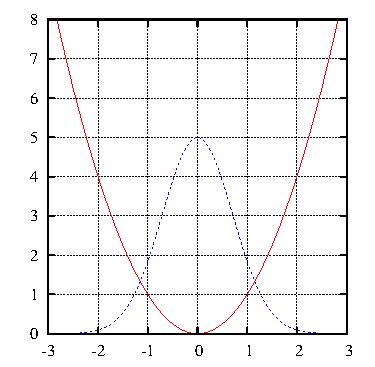
\includegraphics{image/harmonic.pdf}}
\end{frame}

\begin{frame}[t,fragile]{Metropolis法}
  \begin{itemize}
    \setlength{\itemsep}{1em}
  \item 現在の配位$x$から、試行配位(trial configuration) $x'$を$x - \Delta \sim x + \Delta$の一様分布より選ぶ
  \item 確率$\min \Big( 1, \frac{e^{-\beta V(x')}}{e^{-\beta V(x)}} \Big)$で$x'$を採択(accept)。棄却(reject)された場合にはもとの$x$のまま
  \item 物理量の測定 (reject された場合にもカウントする)
  \item 採択確率(acceptance probability)は、$\frac{e^{-\beta V(x')}}{e^{-\beta V(x)}+e^{-\beta V(x')}}$でもよい
  \item 例: \href{https://github.com/todo-group/computer-experiments/blob/master/exercise/monte_carlo/harmonic.c}{example-2-L2/harmonic.c}
  \end{itemize}
\end{frame}

\begin{frame}[t,fragile]{Metropolis法によるシミュレーション}
  \begin{itemize}
    \setlength{\itemsep}{1em}
  \item $\Delta = 0.1$
    
    \vspace*{-2em}\hfill \resizebox{9cm}{!}{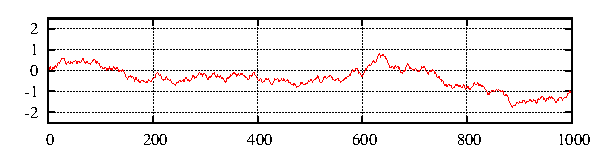
\includegraphics{image/series-001.pdf}}
  \item $\Delta = 1$
    
    \vspace*{-2em}\hfill \resizebox{9cm}{!}{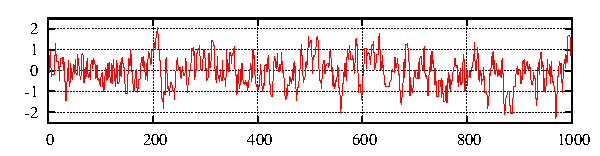
\includegraphics{image/series-010.pdf}}
  \item $\Delta = 10$
    
    \vspace*{-2em}\hfill \resizebox{9cm}{!}{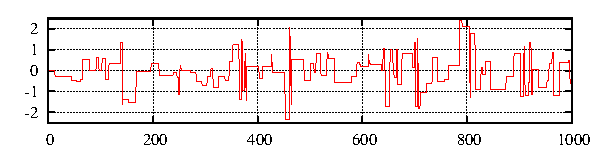
\includegraphics{image/series-100.pdf}}
  \end{itemize}
\end{frame}

\begin{frame}[t,fragile]{自己相関関数(autocorrelation function)}
  \begin{itemize}
    \setlength{\itemsep}{1em}
  \item エルゴード性 + つりあい条件 ⇒ 原理的に正しいマルコフ連鎖モンテカルロ
  \item 実際には自己相関を考慮する必要あり
  \item 自己相関関数
    \[
    C(t) = \frac{\langle A_{i+t}A_i \rangle - \langle A \rangle^2}{\langle A^2 \rangle - \langle A \rangle^2} \sim \exp(-\frac{t}{\tau})
    \]
  \item $\tau$: 自己相関時間(autocorrelation time)
  \item 自己相関の影響により、統計的な「有効サンプル数」が減少
    \[
    M \rightarrow \frac{M}{1+2\tau}
    \]
  \end{itemize}
\end{frame}

\begin{frame}[t,fragile]{自己相関時間と統計誤差}
  \hspace*{4em} 自己相関時間 \hspace*{9em} 統計誤差

  \noindent\resizebox{0.49\textwidth}{!}{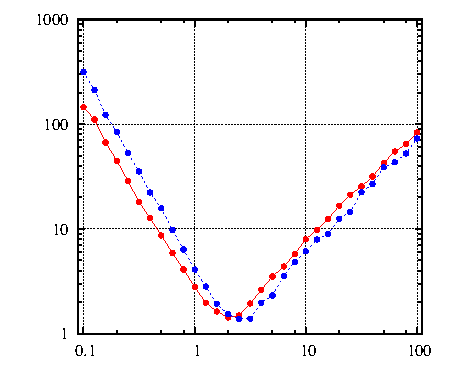
\includegraphics{image/autocorr.pdf}}
  \resizebox{0.49\textwidth}{!}{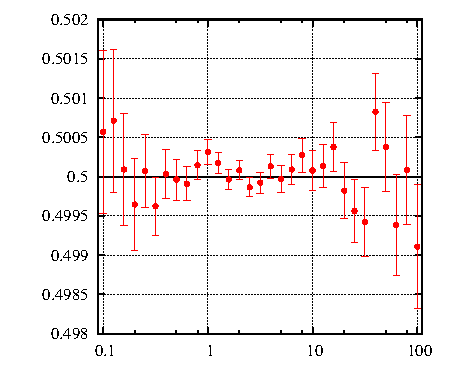
\includegraphics{image/error.pdf}}

  \hspace*{7em} $\Delta$ \hspace*{12em} $\Delta$
\end{frame}

\begin{frame}[t,fragile]{マルコフ連鎖モンテカルロ法}
  \begin{itemize}
    %\setlength{\itemsep}{1em}
  \item 統計誤差はサンプルの生の分散$s^2$とサンプル数$M$、自己相関時間$\tau$で決まる
    \[
    \sigma^2 \simeq \frac{s^2 (1+2\tau)}{M}
    \]
    \begin{itemize}
    \item 一度に大きく配位を動かそうとすると棄却率が増加 $\Rightarrow$ $\tau$が増加
    \item 動かす幅を小さくすると棄却率は高いが相関が消えない $\Rightarrow$ $\tau$が増加
    \item 非局所更新法、拡張アンサンブル法など様々な方法が使われている
    \end{itemize}
  \item 物理以外でも、Bayes推定や機械学習、社会現象のシミュレーションなど広く使われている
  \end{itemize}
\end{frame}

\begin{frame}[t,fragile]{イジング模型に対するモンテカルロ法}
  \begin{itemize}
    %\setlength{\itemsep}{1em}
  \item 更新の単位は一つのスピンとするのが一番自然
  \item メトロポリス法に必要なのは更新前後のエネルギー差だけなので、全エネルギーを計算しなおす必要なし
\begin{verbatim}
for (s = 0; s < num_sites; ++s) {
  delta = 0.0;
  for (j = 0; j < num_neighbors; ++j) {
    v = neighbor(s, j);
    delta += 2 * J * spin[s] * spin[v];
  }
  if (random() < exp(-beta * delta))
    spin[s] = -1 * spin[s];
}  
\end{verbatim}
  \end{itemize}
\end{frame}

\begin{frame}[t,fragile]{物理量の計算}
  \begin{itemize}
    %\setlength{\itemsep}{1em}
  \item 内部エネルギー$E$
    \begin{itemize}
    \item 初期状態のスピンを全て上向き(1)に取ると$E=-J \times \text{ボンド数}$
    \item モンテカルロステップ毎にエネルギーの変化分を計算しているので、採択された場合にはその値を足し込む
    \end{itemize}
  \item 比熱$C$: 内部エネルギーのゆらぎから計算できる
    \[
    C = \frac{1}{N} \frac{\partial E}{\partial T} = \frac{1}{NT^2} (\langle E^2 \rangle - \langle E \rangle^2)
    \]
  \item 磁化$m$: スピンの値の平均値 $m = \frac{1}{N} \sum_i \sigma_i$
    \begin{itemize}
    \item 外部磁場がない場合、対称性から$m$の長時間平均は厳密には零になる
    \item 熱力学極限では対称性が自発的に破れて、低温で有限の$m$
    \item シミュレーションでは$m$ではなく$m^2$を見るとよい
    \end{itemize}
  \end{itemize}
\end{frame}

\begin{frame}[t,fragile]{モンテカルロステップの設定}
  \begin{itemize}
    %\setlength{\itemsep}{1em}
  \item 全てのスピンについて一通り更新を試すのを、1モンテカルロステップと数える
  \item どれくらいのモンテカルロステップが必要かは、あらかじめは分からない
  \item 典型的には、$10^4$---$10^6$程度にとることが多い
  \item 熱平衡化 (thermalization)
    \begin{itemize}
    \item 初期配位依存性を取り除くため、モンテカルロステップの最初の部分は捨てる(burn-in time)
    \item 典型的には、全体の1割程度を捨てることが多い
    \end{itemize}
  \end{itemize}
\end{frame}
